\documentclass[tikz,border=3.14pt]{standalone}
\usepackage{../mymacros}
\usepackage{tikz-3dplot}

\usetikzlibrary{fadings}

\definecolor{poliblue1}{RGB}{93,138,168} 
\definecolor{poliblue2}{RGB}{41,76,113}
\definecolor{poliblue3}{RGB}{25,43,67}
\definecolor{orangep}{RGB}{251,146,116}
\definecolor{redp}{RGB}{245,86,91}
\definecolor{greenp}{RGB}{73,165,150}

\begin{document}
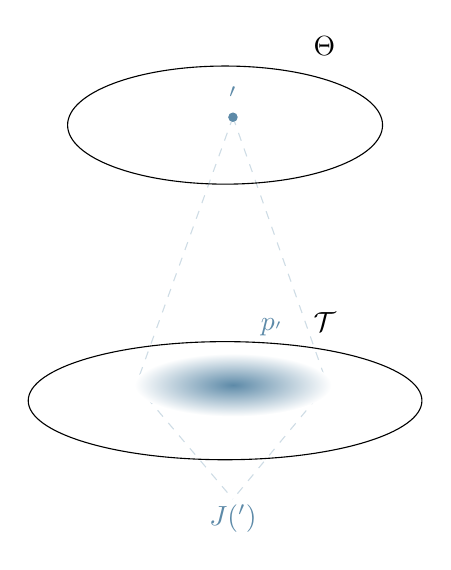
\begin{tikzpicture}[]
\draw[dashed, color=poliblue1, opacity=0.3] (0.1,0.1,0) -- (-1.13,-3.3,0);
\draw[dashed, color=poliblue1, opacity=0.3] (0.1,0.1,0) -- (1.3,-3.3,0);
\draw[] (0,0,0) ellipse (2 and .75) node[right, shift={(1,1)}]{$\Theta$};
\draw [fill, color=poliblue1] (0.1,0.1,0) circle (1.5pt) node[above](a){$\vtheta'$};
\draw[] (0,-3.5,0) ellipse (2.5 and .75) node[right, shift={(1,1)}]{$\mathcal{T}$};
\draw[color=poliblue1] (0.1,-5,0) node (c) {$J(\vtheta')$};
\draw[dashed, color=poliblue1, opacity=0.3](-1.13,-3.3,0) -- (0.1,-4.75,0);
\draw[dashed, color=poliblue1, opacity=0.3] (1.3,-3.3,0) -- (0.1,-4.75,0);
\draw[fill, inner color=poliblue1, outer color=white, draw=none, color=white] (0.1,-3.3,0) ellipse (1.25 and .4) node[above, shift={(.5,.5)}, color=poliblue1]{$p_{\vtheta'}$};
%\draw[dashed, color=poliblue1] (a) -- (-0.7,-3.5,0);
%\draw[->, dashed, color=poliblue1] (-0.7,-3.5,0) -- (c);
\end{tikzpicture}
\end{document}